% Szglab4
% ===========================================================================
%
\chapter{Prototípus koncepciója}

\thispagestyle{fancy}
\setcounter{section}{-1}
\section{Változások a specifikációban}

\subsection{Köd}
\textbf{A tornyokra időnként köd ereszkedik, aminek következtében a látás erősen lecsökken. Ez hatással van a lövésre.}\\
Egy új Fog osztályt vezetünk be. Ennek van egy darab statikus getRangeMultiplier() metódusa, ami visszaadja mennyivel csökkenjen a látótáv, valamint van egy setFog(bool), amivel be lehet állítani, hogy van-e köd vagy nincs. Ha nincs köd beállítva getRangeMultiplier() 1-et ad vissza.

\subsection{Elágazások}
\textbf{A játékosok által járható útvonalon lehetnek elágazások és becsatlakozások. Az elágazásokon az egyes játékosok véletlenszerűen mennek a különböző irányokba.}\\
Mi a feladatot alapból így specifikáltuk, ezért változásra nincs szükség.
\subsection{Új lövedék}
\textbf{A tornyokban elvétve lehetnek olyan lövedékek, amelyek az eltalált játékost kettőbe vágják. A két játékos egymástól függetlenül él tovább, csökkentett életerővel.}\\
Ehhez létrehoztunk egy új SplitterProjectile osztályt, ami a Projectile osztályból származik le. Valamint hozzáadtunk az Enemy osztályhoz egy split() metódust. A Game osztályhoz pedig egy addEnemy(Enemy) metódust adtunk, amit a SplitterProjectile hív meg egy callback-el, amikor kettévágta az ellenséget.

\subsection{Módosult osztálydiagram}
\begin{figure}[H]
\begin{center}
\includegraphics[width=17cm]{images/ch07/class_new_ok.png}
\caption{Osztály diagram}
\label{fig:classDiagNew}
\end{center}
\end{figure}

\subsection{Módosult szekvencia diagramok}
\begin{figure}[H]
\begin{center}
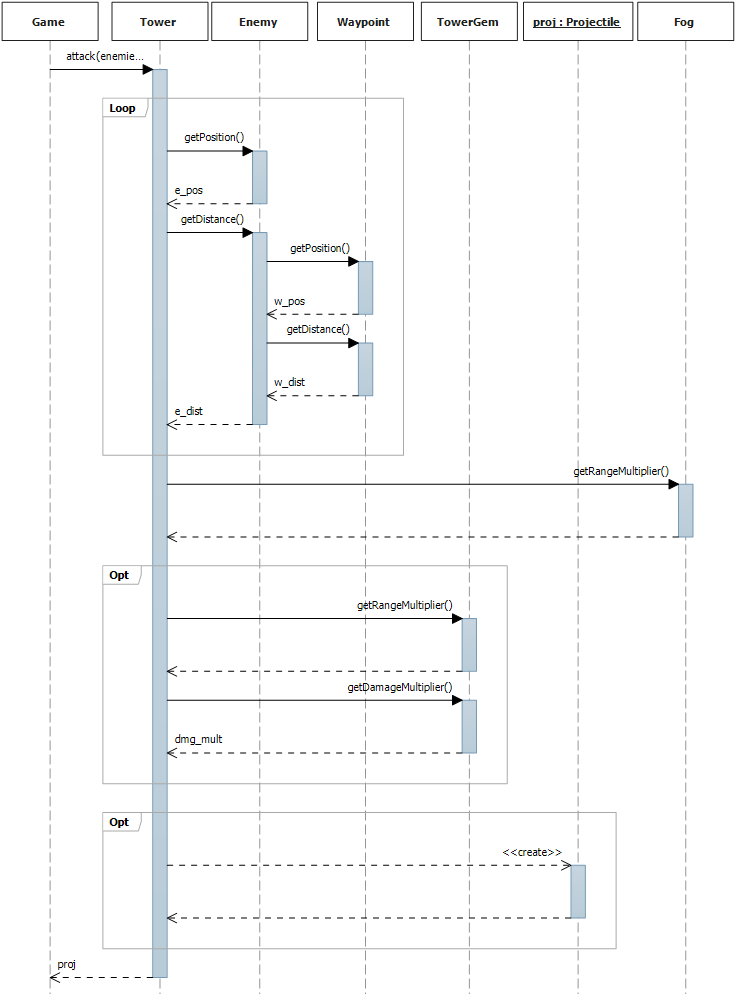
\includegraphics[width=17cm]{images/ch07/attack_enemy.png}
\caption{Ellenség támadása}
\label{fig:enemyAttackNew}
\end{center}
\end{figure}

\begin{figure}[H]
\begin{center}
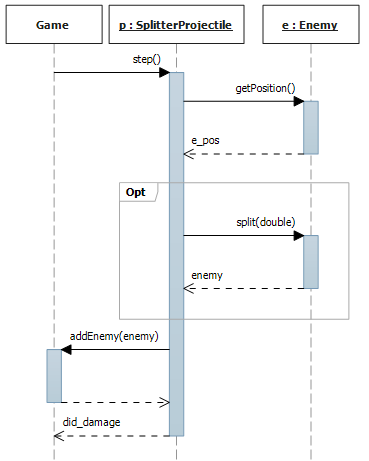
\includegraphics[width=10cm]{images/ch07/splitterprojectile_step.png}
\caption{Újfajta lövedék mozgatása}
\label{fig:splitProjMove}
\end{center}
\end{figure}


\section{Prototípus interface-definíciója}
%\comment{Definiálni kell a teszteket leíró nyelvet. Külön figyelmet kell fordítani arra, hogy ha a rendszer véletlen elemeket is tartalmaz, akkor a véletlenszerűség ki-bekapcsolható legyen, és a program determinisztikusan is tesztelhető legyen.}

\subsection{Az interfész általános leírása}
%\comment{A protó (karakteres) input és output felületeit úgy kell kialakítani, hogy az input fájlból is vehető legyen illetőleg az output fájlba menthető legyen, vagyis kommunikációra csak a szabványos be- és kimenet használható.}

Az interfész csak a szabványos bemenetről fogad parancsokat, és a szabványos kimenetre írja ki az esetleges kimenetet. Ezáltal terminálból is használható, valamint az elkészítendő tesztelő segédprogram segítségével átirányítható a ki- és bemenet fájlokra, így van mód automatikus tesztelésre, előre elkészített teszteseteket felhasználva. A tesztesetek a prototípusnak adandó parancsok sorozatából, valamint az adott sorozatra adandó helyes kimenet található. A tesztek sikeresek, ha a valós, és a leírt elvárt kimenet megegyezik.

\subsection{Bemeneti nyelv}
%\comment{Definiálni kell a teszteket leíró nyelvet. Külön figyelmet kell fordítani arra, hogy ha a rendszer véletlen elemeket is tartalmaz, akkor a véletlenszerűség ki-bekapcsolható legyen, és a program determinisztikusan is futtatható legyen. A szálkezelést is tesztelhető, irányítható módon kell megoldani.}

A prototípus által elfogadott parancsok a következők:

\begin{itemize}

\item loadMap
	\begin{itemize}
	\item Leírás: Egy pálya betöltése
	\item Opciók: A betöltendő pálya neve
	\end{itemize}

\item loadMission
	\begin{itemize}
	\item Leírás: Egy misszió betöltése
	\item Opciók: A betöltendő misszió neve
	\end{itemize}

\item setFog
	\begin{itemize}
	\item Leírás: A köd beállítása
	\item Opciók: A köd kívánt állapota: 0 - nincs köd, 1 - van köd
	\end{itemize}

\item setCritical
	\begin{itemize}
	\item Leírás: A kettévágó lövedék beállítása
	\item Opciók: A kívánt hatás: 0 - nem kettévágó lövedék, 1 - kettévágó lövedék
	\end{itemize}

\item setWaypoint
	\begin{itemize}
	\item Leírás: A csomópontokból való továbbhaladás irányának beállítása
	\item Opciók: A következő csomópont azonosítója
	\end{itemize}

\item step
	\begin{itemize}
	\item Leírás: A játéklogika léptetése
	\item Opciók: A léptetni kívánt időegységek száma
	\end{itemize}

\item buildTower
	\begin{itemize}
	\item Leírás: Toronyépítés
	\item Opciók: Az építendő torony koordinátái
	\end{itemize}

\item buildObstacle
	\begin{itemize}
	\item Leírás: Akadály építése
	\item Opciók: Az építendő akadály koordinátái
	\end{itemize}

\item enchant
	\begin{itemize}
	\item Leírás: Torony vagy akadály felszerelése drágakővel
	\item Opciók: A drágakő típusa, illetve a felszerelendő épület koordinátái
	\end{itemize}

\item listEnemies
	\begin{itemize}
	\item Leírás: A pályán lévő ellenségek kilistázása
	\item Opciók: -
	\end{itemize}

\item listTowers
	\begin{itemize}
	\item Leírás: A tornyok kilistázása
	\item Opciók: -
	\end{itemize}

\item listObstacles
	\begin{itemize}
	\item Leírás: Az akadályok kilistázása
	\item Opciók: -
	\end{itemize}

\item listProjectiles
	\begin{itemize}
	\item Leírás: A lövedékek kilistázása
	\item Opciók: -
	\end{itemize}


\end{itemize}

%\comment{Ha szükséges, meg kell adni a konfigurációs (pl. pályaképet megadó) fájlok nyelvtanát is.}

A pályákat és missziókat leíró fájlok XML formátumban lesznek, a következő DTD-k szerint:\newline
\newline
<!DOCTYPE map\newline
[\newline
<!ELEMENT map (name, waypoint*, route)>\newline
<!ELEMENT name (\#PCDATA)\newline
<!ELEMENT waypoint (id, coords)>\newline
<!ELEMENT id (\#PCDATA)\newline
<!ELEMENT coords (x, y)>\newline
<!ELEMENT x (\#PCDATA)\newline
<!ELEMENT y (\#PCDATA)\newline
<!ELEMENT route (a, b, chance)>\newline
<!ELEMENT a (\#PCDATA)\newline
<!ELEMENT b (\#PCDATA)\newline
<!ELEMENT chance (\#PCDATA)\newline
]>\newline
\newline
<!DOCTYPE mission\newline
[\newline
<!ELEMENT mission (name, enemy*)>\newline
<!ELEMENT name (\#PCDATA)\newline
<!ELEMENT enemy (id, type)>\newline
<!ELEMENT id (\#PCDATA)\newline
<!ELEMENT type (\#PCDATA)\newline
]>\newline

\subsection{Kimeneti nyelv}
%\comment{Egyértelműen definiálni kell, hogy az egyes bemeneti parancsok végrehajtása után előálló állapot milyen formában jelenik meg a szabványos kimeneten.}

Kimenetet csak a következő 4 parancs ad, a következő formában:\newline
\newline
listEnemies\newline
Az összes élő ellenséget írja ki, soronként egyet:\newline
<sorszám> <életerő> <koordináták>\newline
\newline
listTowers\newline
Az összes tornyot írja ki, soronként egyet:\newline
<sorszám> <koordináták> <varázskő>\newline
\newline
listObstacles\newline
Az összes tornyot írja ki, soronként egyet:\newline
<sorszám> <koordináták> <varázskő>\newline
\newline
listProjectiles\newline
Az összes tornyot írja ki, soronként egyet:\newline
<sorszám> <koordináták> <célpont> <szétvágó-e>\newline
\newline
\pagebreak
\section{Összes részletes use-case}
%\comment{A use-case-eknek a részletezettsége feleljen meg a kezelői felületnek, azaz a felület elemeire kell hivatkozniuk.
% Alábbi táblázat minden use-case-hez külön-külön.}

\usecase
{buildObstacle}
{A megadott koordinátákra épít egy akadályt.}
{Tesztelő}
{A kapott koordinátákra megnézi a program, hogy épülhet-e akadály. Ha nem akkor nem épül meg és kiírja, hogy nem épült meg.
Ha igen akkor bekerül az akadály listába egy új akadály a koordinátákkal.}

\usecase
{buildTower}
{A megadott koordinátákra épít egy tornyot.}
{Tesztelő}
{A kapott koordinátákra megnézi a program, hogy épülhet-e torony. Ha nem akkor nem épül meg és kiírja, hogy nem épült meg.
Ha igen akkor bekerül a torony listába egy új torony a koordinátákkal.}

\usecase
{enchant}
{A megadott koordinátán levő toronyra vagy akadályra egy megadott színű varázskövet tesz. }
{Tesztelő}
{Ha a kapott koordinátán van egy akadály vagy torony akkor azt felruházza egy kapott színű varázskővel.}

\usecase
{listEnemies}
{Kilistázza az ellenségeket.}
{Tesztelő}
{Kiírja a kimenetre a játékban levő ellenségeket.}

\usecase
{listObstacles}
{Kilistázza az akadályokat.}
{Tesztelő}
{Kiírja a kimenetre a játékban levő akadályokat.}

\usecase
{listProjectiles}
{Kilistázza a lövedékeket.}
{Tesztelő}
{Kiírja a kimenetre a játékban levő lövedékeket.}

\usecase
{listTowers}
{Kilistázza a tornyokat.}
{Tesztelő}
{Kiírja a kimenetre a játékban levő tornyokat.}

\usecase
{loadMap}
{Betölti a kiválasztott pályát.}
{Tesztelő}
{A bementeten megadott nevű pályát betölti, ha létezik olyan.}

\usecase
{loadMission}
{Betölti a kiválasztott küldetést.}
{Tesztelő}
{A bementeten megadott nevű küldetést betölti, ha létezik olyan.}

\usecase
{setCritical}
{Beállítja, hogy kettévágó lövedékek keletkezzenek-e.}
{Tesztelő}
{Kiveszi a véletlenszerűséget a kettévágó lövedékek keletkezéséből, és egy általunk megadott értékre állítja. (0-1)}

\usecase
{setFog}
{Beállítja, hogy legyen-e köd.}
{Tesztelő}
{Kiveszi a véletlenszerűséget a köd keletkezéséből, és egy általunk megadott értékre állítja. (0-1)}

\usecase
{setWaypoint}
{Beállítja egy útelágazódásnak a következő célállomást.}
{Tesztelő}
{Kiveszi a véletlenszerűséget a következő célállomás kiválasztásából, és egy általunk megadott célállomásra állítja egy ID alapján.}

\usecase
{step}
{Lépteti a programot.}
{Game osztály}
{A tesztelhetőség miatt, egy időzített belső ciklus helyett ezzel lehet egyesével léptetni a program főciklusát,
 amibe beletartozik az ellenségek és lövedékek mozgatása, valamint a küldetés alapján, új ellenségek behozatala.}

\section{Tesztelési terv}

\teszteset
{Ellenség mozgatása (nem érte el a következő Waypoint-ot)} % Teszteset neve
{Ellenségek mozgásának tesztelése.} % Rövid leírás
{Teszteli, hogy az ellenségek megfelelően mozognak-e a cél felé a pályán, ha nem kell Waypoint-ot váltaniuk.} % Teszt célja

\teszteset
{Ellenség mozgatása (elérte a következő Waypoint-ot)}
{Ellenségek mozgásának tesztelése.}
{Teszteli, hogy az ellenségek megfelelően mozognak-e a cél felé a pályán, ha Waypoint-ot kell váltaniuk.}

\teszteset
{Lassítás}
{Az ellenségek lassításának tesztelése.}
{Teszteli, hogy az akadályok megfelelően lassítják-e a hatókörükben lévő ellenségeket, illetve hogy a hatókörükön kívülieket nem befolyásolják.}

\teszteset
{Lassítás varázskővel ellátott akadályokkal}
{Az ellenségek lassításának tesztelése.}
{Teszteli, hogy az varázskővel ellátott akadályok helyesen működnek-e.}

\teszteset
{Lövés}
{A tornyok lövésének tesztelése.}
{Teszteli, hogy a tornyok által kilőtt lövedék elér-e egy ellenséget, és megsebzi-e, illetve hogy a megfelelő időközönként lő-e a torony.}

\teszteset
{Lövés ködben}
{A tornyok lövésének tesztelése.}
{Teszteli, hogy a tornyoknak kisebb lesz-e a hatótávolsága ködben.}

\teszteset
{Lövés varázskővel ellátva}
{A tornyok lövésének tesztelése.}
{Teszteli, hogy a tornyoknak változnak-e a tulajdonságai varázskővel ellátva.}

\teszteset
{Megfelelő célra lövés}
{A tornyok célkiválasztását teszteli.}
{Teszteli, hogy a tornyok a hatókörükben lévő ellenségek közül a célhoz legközelebbire lőnek-e.}

\teszteset
{Lövedék által kettőbe vágás}
{A kettévágó lövedék tesztelése.}
{Teszteli, hogy az ellenségek két részre szakadnak-e a kettévágó lövedék hatására.}

\teszteset
{Toronyépítés}
{Toronyépítés tesztelése.}
{Teszteli, hogy a torony megépül-e egy érvényes helyre és hogy nem lehet megépíteni egy érvénytelen helyre.}

\teszteset
{Akadályépítés}
{Akadályépítés tesztelése.}
{Teszteli, hogy az akadály megépül-e egy érvényes helyre és hogy nem lehet megépíteni egy érvénytelen helyre.}

\teszteset
{Torony varázskővel ellátása}
{Torony varázskővel való ellátásának tesztelése.}
{Teszteli, hogy a jó helyre rakott varázskő rákerül-e a toronyra, a rossz helyre rakott pedig nem.}

\teszteset
{Akadály varázskővel ellátása}
{Akadály varázskővel való ellátásának tesztelése.}
{Teszteli, hogy a jó helyre rakott varázskő rákerül-e az akadályra, a rossz helyre rakott pedig nem.}

\section{Tesztelést támogató segéd- és fordítóprogramok specifikálása}
A tesztelés emberi erővel hosszadalmas, és repetitív, a program működése viszont determinisztikus, így minden feltétel adott, hogy a teszt kiértékelését gép végezze el. A segédprogram teszt bemeneteket tárol, hozzájuk rendelve a várt kimenettel. A segédprogram lefuttatja a megadott tesztet (vagy többet), és összeveti a kimenetüket az elvárt kimenettel (az összehasonlítás szöveges alapon történik, leginkább a UNIX-ban található diff parancshoz lehet hasonlítani). Amennyiben a kimenet nem egyezik meg az elvárt kimenettel, úgy a teszt nem sikerült (fail), ellenkező esetben a teszt sikeres (pass). Hiba esetén a program kijelzi, hogy hol, és milyen eltérést talált.

